\documentclass[a3paper]{ltjsarticle}
%数式
\usepackage{amsmath,amsfonts,multicol}
\usepackage{bm}
\usepackage{graphicx}
\usepackage{tcolorbox}
\usepackage{svg}
\usepackage[margin=5truemm]{geometry}
\usepackage{float}



\setlength{\columnseprule}{.4pt}

\begin{document}
\noindent {\Large{\bf DSP 最終レポート　ActorCritic,Q学習エージェントに対するパラメタ探索、性能比較、最適化}
\begin{multicols*}{2}
    \section*{Intro}
    本レポートでは、MDPGridworld-v3に対して開発した性能の良いエージェント
    について述べる。
    エージェントは、ActorCritic法をベースとして、
    報酬の低いエピソード終了フラグをもつ状態に遷移しないよう、改良を加えたものを使用した。
    \section*{手法}
    \subsection*{Q学習とActorCritic法について}
    まず、Q学習とActorCritic法のエージェントの学習方法の違いから述べる。
    それぞれのエージェントは状態sの時に行動aを行った所、
    報酬rを得て状態s'に遷移したと仮定する。また、$\gamma$は報酬の割引率である。

    Q学習では、行動価値関数Q(s,a)の値を、
    ActorCriticでは状態価値V(s)と方策関数$\pi(s,a)$をそれぞれ以下のように更新する。
    \begin{align*}
         & Q(s,a) \leftarrow Q(s,a)                                                 \\
         & +\alpha
        \{r+\gamma \max_aQ(s',a)-Q(s,a)\}                                           \\
        \\
         & td=r+\gamma V(s')-V(s)                                                   \\
         & V(s)\leftarrow V(s)+\alpha td　\quad\pi (s,a)\leftarrow\pi (s,a)+\beta td
    \end{align*}
    これらの更新式はいずれも、まず、QやVの予測誤差である時間的差分(TD)を計算する。
    予測誤差をもとの関数に足し合わせて更新することにより、Q学習やActorCritic法では
    より正確な値を得ることができる。
    $\alpha,\beta$は任意に決めれるハイ・パラメータで、更新の度合いを決定する。

    次に、状態sの時の行動選択について、Q学習は$\arg\max_aQ(s,a)$を選ぶ。
    ActorCritic法はとれる行動が$[a_1,a_2,a_3]$である時、
    $[\pi(s,a_1),\pi(s,a_2),\pi(s,a_3)]$をsoftmax関数
    に代入して得られた値をその行動をとる確率として選択する。

    \subsection*{ActorCriticに加えた修正}
    MDPGridworld-v3の場合、報酬が高いエピソード終了フラグをもつ状態が一つと
    低い報酬をもつエピソード終了フラグを持つ状態が複数ある。
    今後、前者を真のゴール、後者を偽のゴールと呼ぶ。
    このような環境下では、エージェントは偽のゴールに遷移し、総報酬が低くなる。
    すなわち、局所最適に陥る。
    これを回避するため、偽のゴール以上、真のゴール以下の値を持つ
    閾値$r_{threshold}$を設定し、
    $r<r_{threshold}$の時、$td\leftarrow -1000$と、非常に低い値を代入する。
    こうすることで、偽のゴールへ至ることを回避している。

    \section*{Results}
    \subsection*{Q学習とActorCritic法の最適パラメータの探索}
    エージェントを動かすにあたって、ハイ・パラメータを設定する必要がある。
    この設定によって、そのエージェントの性能は大きく変わりうるため、
    実際に総報酬が多くなるようなハイ・パラメータの探索をする必要がある。

    次に、パラメータの探索範囲について述べる。
    Q学習では、割引率$\gamma$とランダムに行動選択をする確率$\epsilon$がそれぞれ
    [0.2,0.5,0.8]の値をとるとして探索を行った。$\alpha$は0.2で固定した。
    一方、ActorCritic学習では、$\alpha,\beta$がそれぞれ[0.2,0.5,0.8]の値をとるとして探索を行った。
    $\gamma$は0.95で固定した。
    こうして探索した結果が、以下の図である。
    \newcommand{\figcm}{5cm}
    \begin{figure}[H]
        \centering
        \begin{minipage}{0.4\columnwidth}
            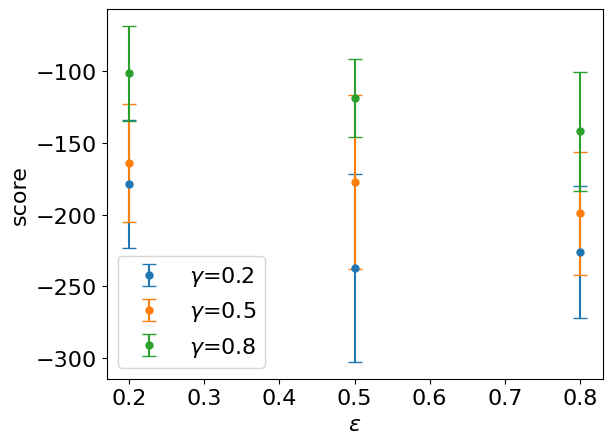
\includegraphics[width=\figcm]{Q_params.png}
            \caption{Q学習のパラメタ探索}
        \end{minipage}
        \begin{minipage}{0.4\columnwidth}
            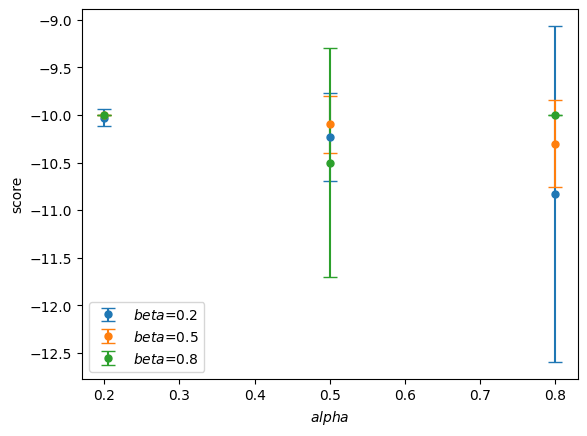
\includegraphics[width=\figcm]{ActorCritic_params.png}
            \caption{ActorCritic法のパラメタ探索}
        \end{minipage}
    \end{figure}
    各エージェントに100回のエピソードを学習させながら行わせ、最後の10回のエピソードの総報酬の平均と分散を求めた。
    この最後の10エピソードの平均と分散を表す。
    Q学習の場合、$\epsilon=0.2,\gamma=0.8$の場合が最も平均が高いので、これを最適パラメータとみなす。
    ActorCritic法の場合、平均の差は小さいので分散の大きさを評価対象とする。
    分散が大きい、すなわち環境の探索性能が高い$\alpha=0.8,\beta=0.2$を最適方策とする

    \subsection*{Q学習とActorCritic法の比較}
    前節で決定した最適パラメータを使ったエージェントに対し、学習を
    行わせた。エピソードごとのステップ数と総報酬を下図に示す。
    \begin{figure}[H]
        \centering
        \begin{minipage}{0.4\columnwidth}
            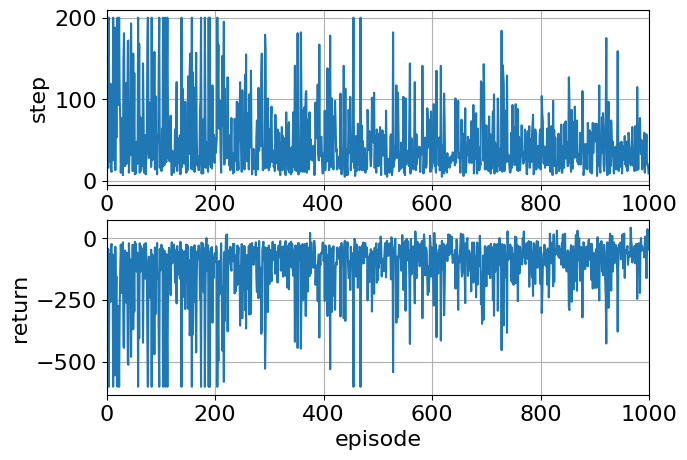
\includegraphics[width=\figcm]{Q.png}
            \caption{Q学習のスコアとステップ}
        \end{minipage}
        \begin{minipage}{0.4\columnwidth}
            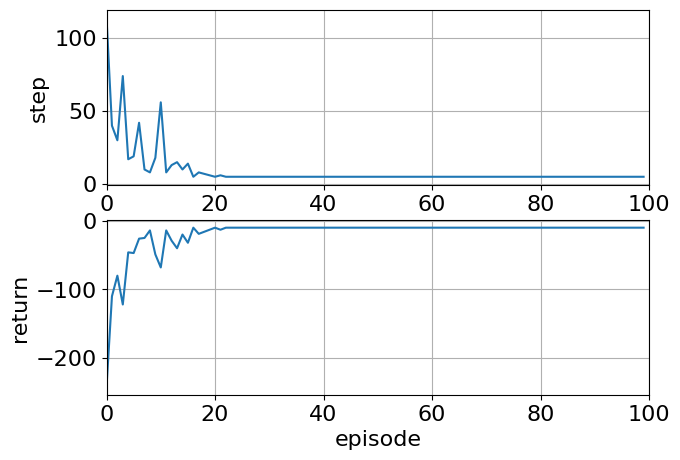
\includegraphics[width=\figcm]{ActorCritic.png}
            \caption{ActorCriticのスコアとステップ}
        \end{minipage}
    \end{figure}
    ActorCriticエージェントは20エピソード目程度で学習が収束するのに
    対し、Qエージェントはいつまでたっても収束くしない。
    ActorCriticエージェントの方ががより良いエージェントといえる。

    \subsection*{修正されたActorCritic法の性能評価}
    前節のActorCriticエージェントは、総報酬が-10に収束した。
    この環境において、最適方策をとった場合の総報酬は58なので、局所最適に陥っている。
    修正されたActorCriticエージェントの学習の様子を以下に示す。
    \begin{figure}[H]
        \centering
        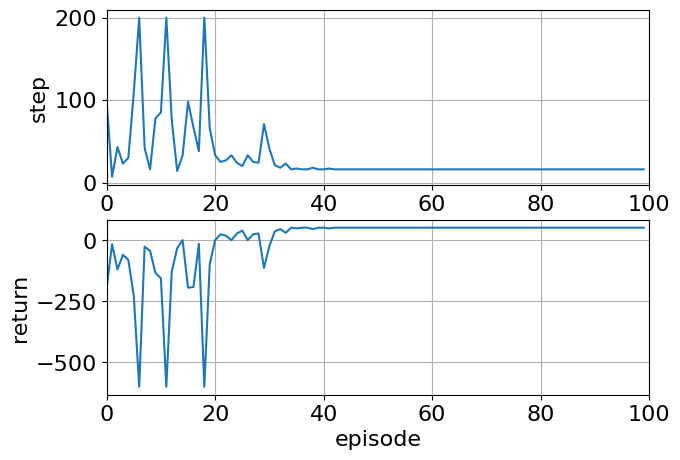
\includegraphics[width=\figcm]{ActorCritic_advanced.png}
        \caption{修正されたActorCritic法}
    \end{figure}
    総報酬は52に収束した。修正を加えることで、確かに最適方策
    に近い方策を得ることができた。
    \section*{Discussion}
    Q学習エージェントは$s\times a$個、ActorCriticエージェントは$s\times a+s$個分の
    実数値情報を記憶している。(s:状態の個数、a:行動の個数)
    ActorCriticはQ学習と比較し、環境に対しより多くの記憶容量を持っているため、より優れた学習性能を発揮したと考えられる。

    また、ActorCriticに対する修正は、真のゴールが持つ報酬が分かっていることを前提としていた。
    このように環境に対する仮定を加えると、エージェントの性能はよくなることが分かる。
\end{multicols*}
\end{document}